%% genome_scale_prediction.tex
%% Author: Leighton Pritchard
%% Copyright: James Hutton Institute
%% A brief description of functional annotation

%% trip_to_the_doctor.tex
%% Author: Leighton Pritchard
%% Copyright: James Hutton Institute
%% A brief example to demonstrate the importance of accounting for multiple-testing

% SUBSECTION: a short aside
\subsection{A visit to the doctor}

\begin{frame}
  \frametitle{A wee trip to the doctor}
  \begin{itemize}
    \item<1-> You go for a checkup, and are tested for disease $X$
    \item<1-> The test has \textbf{$\text{sensitivity}=0.95$} (predicts disease where there is disease)
    \item<1-> The test has \textbf{$\text{FPR}=0.01$} (predicts disease where there is no disease)
    \item<2-> Your test is \emph{positive}
    \item<2-> \textbf{What is the probability that you have disease $X$?}
    \begin{itemize}
      \item \textbf{0.01, 0.05, 0.50, 0.95, 0.99?}
    \end{itemize}
    \item<2-> (Audience Participation!)
  \end{itemize} 
\end{frame}

\begin{frame}
  \frametitle{A wee trip to the doctor}
  \begin{itemize}
    \item<1-> What is the probability that you have disease $X$?
    \item<1-> \textbf{Unless you know the \emph{baseline occurrence} of disease $X$, you cannot determine this.}
    \item<2-> Baseline occurrence: $f_X$
    \begin{itemize}
      \item $f_X = 0.01 \implies P(\text{disease}|\text{+ve}) = 0.490 \approx 0.5$
      \item $f_X = 0.8 \implies P(\text{disease}|\text{+ve}) = 0.997 \approx 1.0$         
    \end{itemize}
  \end{itemize} 
\end{frame}





% SUBSECTION: Genome-scale prediction
\subsection{Statistics of genome-scale prediction}
\begin{frame}
  \frametitle{Why Performance Metrics Matter\footnote{\tiny{\href{http://dx.doi.org/10.1007/978-1-62703-986-4_4}{Pritchard and Broadhurst (2014) \textit{Methods Mol. Biol.} \textbf{1127}:53-64 doi:10.1007/978-1-62703-986-4\_4}}}}
  \begin{itemize}
    \item<1-> Imagine a predictor for protein functional class (e.g. Type III effector)
    \item<1-> The paper reports \textbf{$\text{sensitivity}=0.95$}, \textbf{$\text{FPR}=0.01$}
    \item<1-> You run the predictor on 20,000 proteins in an organism
    \item<1-> It predicts 130 members of the class. How many of them are likely to be true positives?
    \item<2-> \textit{We need a baseline level of that class in the genome to determine this.}        
    \item<2-> We estimate $\approx$ 200 members in protein complement, so $f_X=0.01$
    \begin{itemize}
      \item $f_X = 0.01 \implies P(\text{class}|\text{+ve}) = 0.490 \approx 0.5$
    \end{itemize}
  \end{itemize} 
\end{frame}

\begin{frame}
  \frametitle{Bayes' Theorem}
  \begin{itemize}
    \item May seem counter-intuitive: 95\% sensitivity, 99\% specificity $\implies$ \textbf{50\% chance} of any prediction being incorrect
    \item Probability given by Bayes' Theorem
    \begin{itemize}
      \item $P(X|+) =  \frac{P(+|X) P(X)}{P(+|X) P(X) + P(+|\bar{X}) P(\bar{X})}$
    \end{itemize}
    \item This step commonly overlooked in the literature (confirmation bias? people want to see positives/their predictor work)
  \end{itemize} 
\end{frame}

\begin{frame}
  \frametitle{A cautionary tale\footnote{\tiny{\href{http://dx.doi.org/10.1371/journal.ppat.1000376}{Arnold \textit{et al}. (2009) \textit{PLoS Pathog.} \textbf{5}:e1000376 doi:10.1371/journal.ppat.1000376}}}}
  \begin{itemize}
    \item<1-> Paper describes \textbf{EffectiveT3}, a type III effector prediction tool
    \item<1-> Reported \textbf{sensitivity $\approx$ 0.71, FPR $\approx$ 0.15}
    \item<1-> Applied tool to 739 complete bacterial and archaeal genomes
    \item<2-> Organisms with an identifiable T3SS: 2-7\% of genome predicted to be secreted
    \item<2-> \textbf{Organisms without an identifiable T3SS (or known not to have one): 1-10\% of genome predicted to be secreted}
    \item<2-> ``\textit{The surprisingly high number of (false) positives in genomes without T3SS exceeds the expected false positive rate}''
    \item<2-> This is not a surprise, statistically.
  \end{itemize} 
\end{frame}

\begin{frame}
  \frametitle{A cautionary tale\footnote{\tiny{\href{http://dx.doi.org/10.1371/journal.ppat.1000376}{Arnold \textit{et al}. (2009) \textit{PLoS Pathog.} \textbf{5}:e1000376 doi:10.1371/journal.ppat.1000376}}}}
    Probability that an \texttt{EffectiveT3} positive prediction corresponds to a secreted protein is given by Bayes' Theorem \\[0.2cm]
    \begin{itemize}
      \item $P(X|+) =  \frac{P(+|X) P(X)}{P(+|X) P(X) + P(+|\bar{X}) P(\bar{X})}$
      \begin{itemize}
        \item $P(+|X)$ = sensitivity = 0.71
        \item $P(+|\bar{X})$ = FPR = 0.15
        \item $P(X)$ = base rate $\approx$ 0.03 $^($\footnote{\tiny{\href{http://dx.doi.org/10.1146/annurev-phyto-080508-081936}{Boch and Bonas (2010) \textit{Annu. Rev. Phytopathol.} \textbf{48}:419-436 doi:10.1146/annurev-phyto-080508-081936}}}$^)$
        \item $\implies P(X|+) \approx 0.13$
      \end{itemize}
    \end{itemize}
  How many predicted type III secreted proteins were there$\ldots$
\end{frame}

\begin{frame}
  \frametitle{A cautionary tale\footnote{\tiny{\href{http://dx.doi.org/10.1371/journal.ppat.1000376}{Arnold \textit{et al}. (2009) \textit{PLoS Pathog.} \textbf{5}:e1000376 doi:10.1371/journal.ppat.1000376}}}}
  \begin{center}
    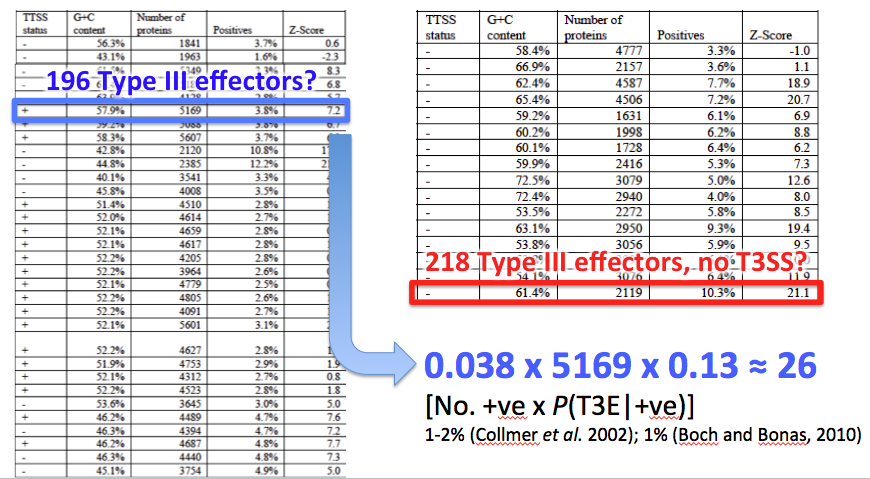
\includegraphics[height=0.65\textheight]{images/arnold_results}  
  \end{center}
\end{frame}

\begin{frame}
  \frametitle{Interpreting genome-scale predictions\footnote{\tiny{\href{http://dx.doi.org/10.1007/978-1-62703-986-4_4}{Pritchard and Broadhurst (2014) \textit{Methods Mol. Biol.} \textbf{1127}:53-64 doi:10.1007/978-1-62703-986-4\_4}}}}
  \begin{itemize}
    \item<1-> Statistics at genome-scale can be counterintuitive.
    \item<1-> \textbf{Use Bayes' Theorem!}
    \item<1-> Predictions identify groups, not individual members of the group. e.g.
    \begin{itemize}
      \item Test for airport smugglers has $P(\text{smuggler}|+) = 0.9$
      \item Test gives 100 positives
    \end{itemize}
    \item<1-> Which specific individuals are truly smugglers?
    \item<2-> The test \emph{does not} allow you to determine this - you need more evidence for each individual
    \item<2->  Same principle applies to other classifiers, (including protein functional class prediction) - watch for `cherry-picking' in publications
  \end{itemize} 
\end{frame}